\chaptercustom{4}{THIẾT KẾ HƯỚNG ĐỐI TƯỢNG}

Chương này trình bày thiết kế hướng đối tượng của Asymptotic dựa trên mô hình phân tích ở Chương 3. Khác với chương phân tích, chương thiết kế được phép đưa các lớp service, repository, adapter, handler, package, trạng thái, dữ liệu và giao diện API để làm rõ cách hệ thống có thể được triển khai thành một nguyên mẫu backend.

\section{Kiến trúc tổng thể}

Asymptotic được thiết kế như một Gateway tài chính thời gian thực đặt giữa AI Agent bên ngoài và các nhà cung cấp dịch vụ AI trả phí. Mỗi request do Agent gửi vào phải đi qua Gateway để được xác thực, kiểm tra chính sách, kiểm tra ngân sách, định tuyến tới provider bằng credential nội bộ và ghi nhận usage/cost/trace.

Ở mức kiến trúc, hệ thống được tổ chức theo mô hình modular monolith kết hợp kiến trúc phân lớp. Các module nghiệp vụ chạy trong cùng một tiến trình triển khai, phối hợp qua lời gọi nội bộ và sử dụng một cơ sở dữ liệu vật lý chung; ranh giới module được duy trì bằng interface và quyền sở hữu dữ liệu ở mức logic. Lựa chọn này phù hợp với phạm vi MVP vì các nghiệp vụ tài chính như tạm giữ ngân sách, quyết toán chi phí, hoàn trả phần dư, nạp tiền và phân bổ ngân sách cần tính nhất quán mạnh trong cùng một backend. Nếu tách sớm thành nhiều service độc lập, hệ thống sẽ phải xử lý giao dịch phân tán, retry, ordering và đối soát phức tạp hơn phạm vi đồ án.

\begin{description}
    \item[Presentation Layer] Tiếp nhận request từ AI Agent, quản trị viên, lập trình viên và Payment Provider. Lớp này xử lý giao tiếp HTTP, kiểm tra định dạng đầu vào và chuyển yêu cầu vào tầng ứng dụng.
    \item[Application Layer] Điều phối các use case bằng service ứng dụng cho request AI, cơ cấu tổ chức, Agent, API key, ngân sách, ví và báo cáo.
    \item[Domain Layer] Chứa các thực thể và quy tắc nghiệp vụ về cơ cấu tổ chức, Agent, khóa truy cập, hạn mức bốn cấp, giao dịch tài chính, provider, model và trace.
    \item[Infrastructure Layer] Hiện thực repository trên cơ sở dữ liệu dùng chung, adapter gọi AI Provider, adapter thanh toán, hashing API key, transaction boundary và cấu hình hạ tầng.
\end{description}

Gateway là điểm cưỡng chế tài chính của hệ thống. Một request chỉ được gọi tới AI Provider sau khi API key hợp lệ, Agent còn hoạt động, policy cho phép, ngân sách đủ điều kiện và hệ thống đã có bản ghi để truy vết hoặc đối soát.

\section{Thiết kế gói}

Thiết kế gói chia hệ thống thành các module theo tầng kiến trúc và miền trách nhiệm. Các gói presentation phụ thuộc vào application service; application service sử dụng domain model và các cổng hạ tầng; domain model không phụ thuộc ngược lại vào framework, cơ sở dữ liệu hoặc provider bên ngoài.

\begin{figure}[H]
    \centering
    
\includegraphics[width=0.95\textwidth,height=0.78\textheight,keepaspectratio]{report_support_documentation/diagrams/chapter_4/package/diagram.png}
    \caption[Biểu đồ gói hệ thống]{Biểu đồ gói hệ thống Asymptotic}\label{fig:package-diagram}
\end{figure}

\cref{fig:package-diagram} thể hiện bốn tầng chính và các gói nghiệp vụ: identity, organization structure, agent, apikey, policy, ledger, provider catalog, payment và reporting. Đây là các module logic trong cùng một ứng dụng modular monolith, không phải các microservice có cơ sở dữ liệu riêng.

\begin{longtable}{|L{0.22\textwidth}|L{0.24\textwidth}|L{0.44\textwidth}|}
\caption{Các package chính trong thiết kế hệ thống}\\
\hline
\textbf{Package} & \textbf{Tầng chính} & \textbf{Trách nhiệm thiết kế} \\
\hline
\endfirsthead
\hline
\textbf{Package} & \textbf{Tầng chính} & \textbf{Trách nhiệm thiết kế} \\
\hline
\endhead
\texttt{gateway api} & Presentation & Tiếp nhận request AI từ Agent, gọi application service và trả response hoặc lỗi nghiệp vụ.\\
\hline
\texttt{admin api} & Presentation & Tiếp nhận thao tác quản trị tổ chức, Agent, API key, ví, ngân sách, provider và báo cáo.\\
\hline
\texttt{payment callback} & Presentation & Nhận callback hoặc kết quả thanh toán từ Payment Provider.\\
\hline
\texttt{identity} & Application & Quản lý tổ chức, người dùng, vai trò và phạm vi quyền.\\
\hline
\texttt{organization structure} & Application & Quản lý đội ngũ, quan hệ thành viên, lập trình viên và quan hệ sở hữu Agent trong tổ chức.\\
\hline
\texttt{agent} & Application & Đăng ký, cập nhật trạng thái và quản lý thông tin AI Agent bên ngoài.\\
\hline
\texttt{apikey} & Application & Sinh, băm, xác thực, thu hồi và theo dõi trạng thái API key của Agent.\\
\hline
\texttt{policy} & Application & Kiểm tra quota, budget, policy và điều kiện sử dụng trước khi request được route.\\
\hline
\texttt{ledger} & \makecell[l]{Application/\\Domain} & Quản lý ví, tạm giữ ngân sách, quyết toán, bút toán và giao dịch tài chính.\\
\hline
\texttt{provider catalog} & Application & Quản lý provider, model, endpoint, biểu giá và credential nội bộ.\\
\hline
\texttt{payment} & \makecell[l]{Application/\\Infrastructure} & Khởi tạo top-up, xác thực kết quả thanh toán và cập nhật ví tổ chức.\\
\hline
\texttt{reporting} & Application & Tổng hợp usage, cost, transaction và trace theo quyền truy cập.\\
\hline
\texttt{persistence} & Infrastructure & Hiện thực repository, ranh giới transaction và truy cập một cơ sở dữ liệu vật lý dùng chung.\\
\hline
\texttt{provider adapter} & Infrastructure & Chuyển đổi request/response giữa mô hình nội bộ và AI Provider.\\
\hline
\texttt{payment adapter} & Infrastructure & Tích hợp Payment Provider ở mức nguyên mẫu hoặc mô phỏng.\\
\hline
\end{longtable}

\section{Thiết kế lớp}

Từ mô hình BCE ở Chương 3, thiết kế lớp bổ sung các lớp triển khai cần thiết: handler ở tầng presentation, service ở tầng application, entity ở tầng domain, repository và adapter ở tầng infrastructure. Các lớp thiết kế không sao chép toàn bộ codebase mà tập trung vào các lớp có vai trò kiến trúc và nghiệp vụ chính.

\begin{figure}[H]
    \centering
    
\includegraphics[width=0.95\textwidth,height=0.78\textheight,keepaspectratio]{report_support_documentation/diagrams/chapter_4/design_classes/overview.png}
    \caption[Biểu đồ lớp thiết kế tổng quát]{Biểu đồ lớp thiết kế tổng quát của hệ thống}\label{fig:design-class-overview}
\end{figure}

\cref{fig:design-class-overview} cho thấy cách các lớp phân tích được chuyển sang thiết kế. Các lớp boundary được hiện thực thành handler, các lớp control được hiện thực thành service, còn các lớp entity tiếp tục là domain entity. OrganizationStructureService quản lý Team, TeamMembership và DeveloperProfile; AgentService bảo đảm Developer là chủ thể đăng ký và quản lý Agent. Repository và adapter được bổ sung để cô lập truy cập dữ liệu và tích hợp hệ thống ngoài.

\begin{figure}[H]
    \centering
    
\includegraphics[width=0.98\textwidth,height=0.72\textheight,keepaspectratio]{report_support_documentation/diagrams/chapter_4/design_classes/gateway_request_flow.png}
    \caption[Biểu đồ lớp thiết kế luồng Gateway Request]{Biểu đồ lớp thiết kế cho luồng Gateway Request}\label{fig:design-class-gateway-request}
\end{figure}

\cref{fig:design-class-gateway-request} tập trung vào UC01. GatewayHandler không tự xử lý toàn bộ nghiệp vụ mà gọi AIRequestService. Service này điều phối APIKeyService, IdempotencyService, PolicyService, BudgetReservationService, ProviderRouter, ProviderAdapter, SettlementService và TraceService. Thiết kế này bảo đảm request không thể bỏ qua bước kiểm soát định danh, lũy đẳng, policy và ngân sách.

\begin{figure}[H]
    \centering
    
\includegraphics[width=0.98\textwidth,height=0.55\textheight,keepaspectratio]{report_support_documentation/diagrams/chapter_4/design_classes/finance_ledger.png}
    \caption[Biểu đồ lớp thiết kế tài chính và ledger]{Biểu đồ lớp thiết kế cho tài chính và ledger}\label{fig:design-class-finance-ledger}
\end{figure}

\cref{fig:design-class-finance-ledger} làm rõ phần tài chính của Gateway. WalletService xử lý số dư ví, BudgetAllocationService phân bổ hoặc thu hồi ngân sách, BudgetReservationService tạm giữ ngân sách cho request AI, TransactionService quản lý trạng thái giao dịch và LedgerService ghi nhận bút toán. Các thao tác làm thay đổi tiền đều đi qua transaction và ledger để có thể đối soát.

\section{Thiết kế tương tác}

Thiết kế tương tác mô tả thứ tự phối hợp giữa actor, handler, service, repository, adapter và hệ thống ngoài. Ba sequence diagram được ưu tiên tương ứng với các luồng quan trọng nhất: AI Agent gọi Gateway, đăng ký AI Agent và nạp tiền/phân bổ ngân sách.

\begin{figure}[H]
    \centering
    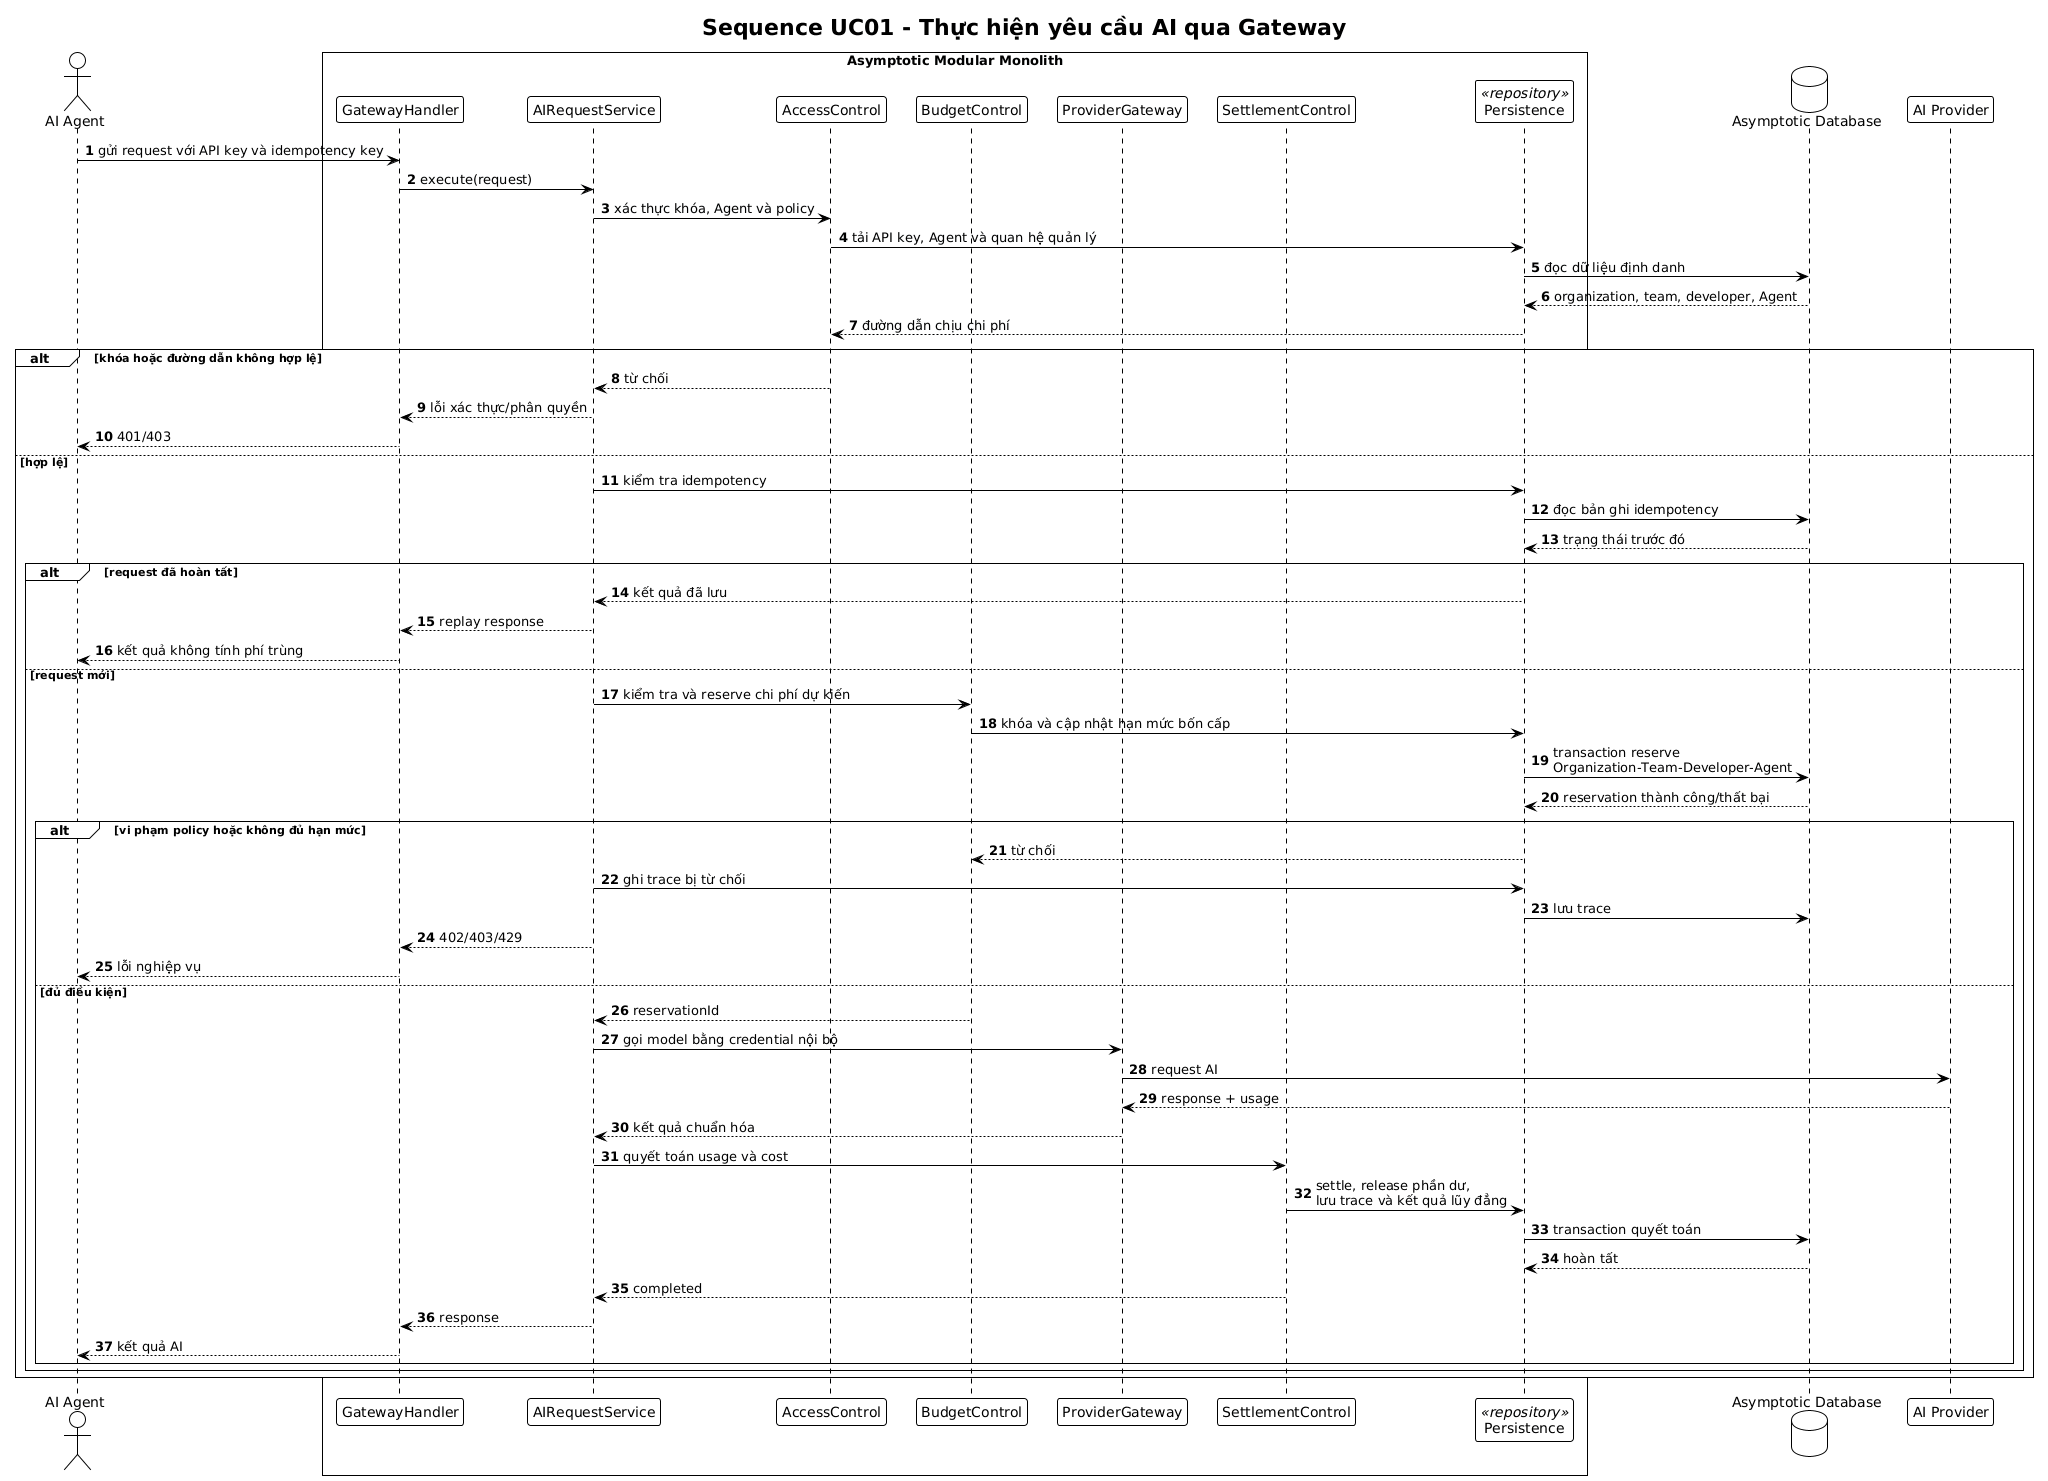
\includegraphics[width=0.98\textwidth,height=0.78\textheight,keepaspectratio]{report_support_documentation/diagrams/chapter_4/sequences/UC01/sequence.png}
    \caption[Biểu đồ tuần tự UC01]{Biểu đồ tuần tự UC01 -- Thực hiện yêu cầu AI qua Gateway}\label{fig:sequence-uc01}
\end{figure}

\cref{fig:sequence-uc01} thể hiện luồng runtime của request AI. Nhánh lỗi quan trọng gồm API key không hợp lệ, request lũy đẳng đã xử lý, vi phạm policy hoặc không đủ ngân sách. Trong nhánh thành công, Gateway gọi AI Provider bằng credential nội bộ thông qua ProviderAdapter, sau đó quyết toán usage/cost và lưu trace.

\begin{figure}[H]
    \centering
    
\includegraphics[width=0.98\textwidth,height=0.64\textheight,keepaspectratio]{report_support_documentation/diagrams/chapter_4/sequences/UC04_agent_registration/sequence.png}
    \caption[Biểu đồ tuần tự đăng ký AI Agent]{Biểu đồ tuần tự đăng ký AI Agent bên ngoài}\label{fig:sequence-agent-registration}
\end{figure}

\cref{fig:sequence-agent-registration} làm rõ Developer là chủ thể đăng ký AI Agent bên ngoài. Hệ thống kiểm tra quan hệ thành viên và phạm vi tổ chức, tạo Agent ở trạng thái chưa kích hoạt rồi gắn Agent với Developer quản lý. Việc cấp hạn mức và cấp API key lần lượt thuộc UC03 và UC05, không được thực hiện ngầm trong UC04.

\begin{figure}[H]
    \centering
    
\includegraphics[width=0.98\textwidth,height=0.70\textheight,keepaspectratio]{report_support_documentation/diagrams/chapter_4/sequences/finance_budget/sequence.png}
    \caption[Biểu đồ tuần tự nạp tiền và phân bổ ngân sách]{Biểu đồ tuần tự nạp tiền và phân bổ ngân sách}\label{fig:sequence-finance-budget}
\end{figure}

\cref{fig:sequence-finance-budget} mô tả chuỗi tương tác tài chính trước khi Agent phát sinh chi phí. Top-up được ghi nhận qua PaymentTransaction, ví tổ chức được cộng tiền sau khi callback hợp lệ, sau đó hạn mức được phân bổ theo các quan hệ liền kề: tổ chức cho đội ngũ, đội ngũ cho Developer và Developer cho Agent. Team, Developer và Agent là các cấp hạn mức trên cùng ví tổ chức, không phải các ví độc lập.

\section{Thiết kế trạng thái}

Các đối tượng có trạng thái quan trọng nhất trong hệ thống là AI Request và Financial Transaction. State machine giúp kiểm tra rằng hệ thống có trạng thái kết thúc rõ cho cả luồng thành công, bị từ chối, lỗi provider và cần đối soát.

\begin{figure}[H]
    \centering
    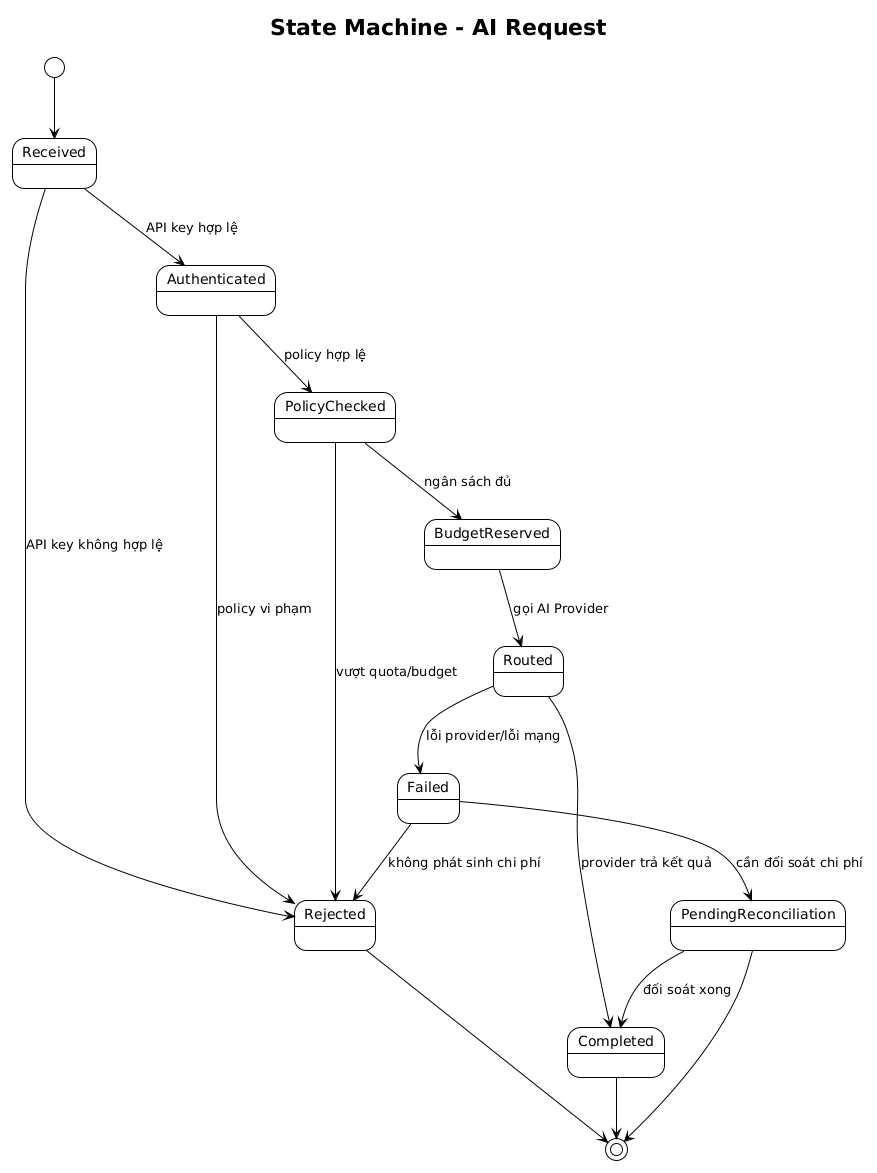
\includegraphics[width=0.86\textwidth,height=0.72\textheight,keepaspectratio]{report_support_documentation/diagrams/chapter_4/states/ai_request_state.png}
    \caption[Biểu đồ trạng thái AI Request]{Biểu đồ trạng thái của AI Request}\label{fig:state-ai-request}
\end{figure}

\cref{fig:state-ai-request} cho thấy request bắt đầu ở trạng thái Received, sau đó chỉ được chuyển tới Routed khi đã xác thực, kiểm tra policy và giữ ngân sách. Request có thể kết thúc ở Completed, Rejected hoặc PendingReconciliation tùy kết quả xử lý.

\begin{figure}[H]
    \centering
    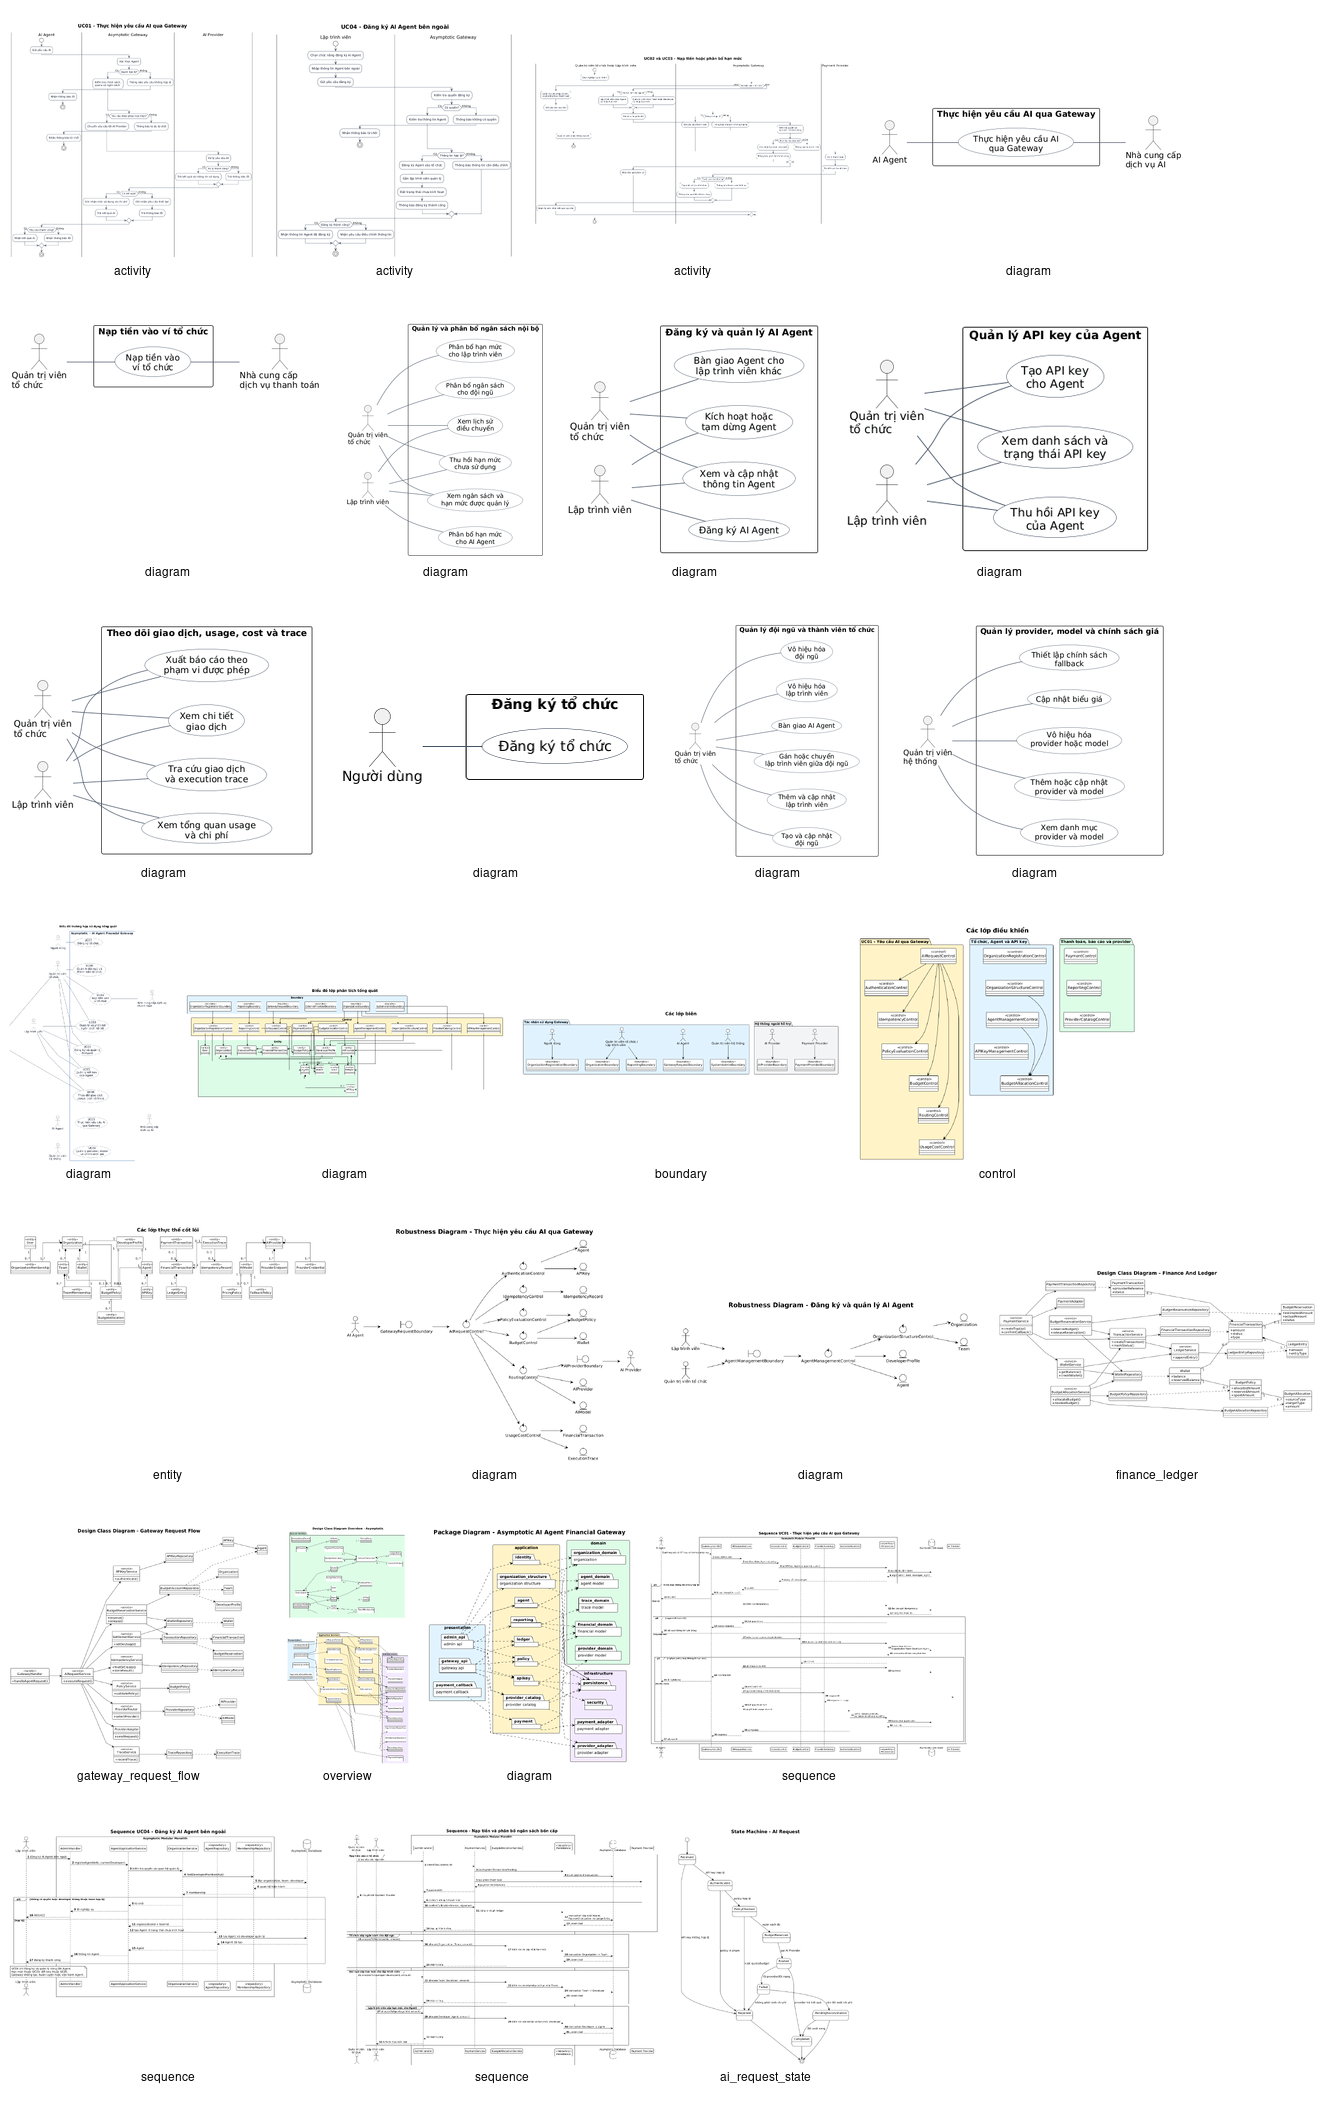
\includegraphics[width=0.92\textwidth,height=0.66\textheight,keepaspectratio]{report_support_documentation/diagrams/chapter_4/states/financial_transaction_state.png}
    \caption[Biểu đồ trạng thái giao dịch tài chính]{Biểu đồ trạng thái của giao dịch tài chính}\label{fig:state-financial-transaction}
\end{figure}

\cref{fig:state-financial-transaction} mô tả vòng đời giao dịch tài chính. Trạng thái Reserved dùng cho khoản tạm giữ trước khi gọi provider; Settled dùng cho giao dịch đã quyết toán; Released dùng khi phần giữ chỗ được giải phóng; PendingReconciliation dùng cho lỗi cần kiểm tra lại để tránh sai lệch tài chính.

\section{Thiết kế dữ liệu và giao diện API}

Thiết kế dữ liệu bám theo các thực thể phân tích ở Chương 3, nhưng được diễn giải ở mức triển khai backend. Các bảng chính được chia theo nhóm nghiệp vụ để phục vụ tính nhất quán tài chính, bảo mật khóa và truy vết request. Mọi module lưu dữ liệu trong một cơ sở dữ liệu vật lý chung; transaction có thể bao phủ các cập nhật liên module cần tính nguyên tử.

\subsection*{Thiết kế dữ liệu}

\begin{longtable}{|L{0.28\textwidth}|L{0.62\textwidth}|}
\caption{Nhóm dữ liệu chính của hệ thống}\\
\hline
\textbf{Nhóm dữ liệu} & \textbf{Nội dung thiết kế} \\
\hline
\endfirsthead
\hline
\textbf{Nhóm dữ liệu} & \textbf{Nội dung thiết kế} \\
\hline
\endhead
Organization, Team, TeamMembership, User, DeveloperProfile & Lưu tổ chức, đội ngũ, danh tính người dùng, vai trò và quan hệ thành viên. Mỗi Developer thuộc tối đa một Team tại một thời điểm trong phạm vi MVP.\\
\hline
Agent & Lưu AI Agent bên ngoài do Developer đăng ký, Developer quản lý hiện tại, trạng thái kích hoạt và phạm vi tổ chức.\\
\hline
APIKey & Lưu khóa truy cập do Asymptotic cấp riêng cho Agent trong UC05. Khóa lưu dạng hash hoặc dạng bảo vệ, có trạng thái active/revoked và thời điểm tạo/thu hồi.\\
\hline
Wallet, BudgetPolicy, BudgetAllocation, BudgetReservation & Wallet lưu tiền thật của tổ chức. Các thực thể còn lại lưu hạn mức bốn cấp, lịch sử phân bổ hoặc thu hồi và khoản tạm giữ cho request AI; chúng không tạo ví độc lập cho Team, Developer hoặc Agent.\\
\hline
FinancialTransaction, LedgerEntry, PaymentTransaction & Lưu giao dịch tài chính, bút toán append-only và giao dịch với Payment Provider. LedgerEntry giúp truy nguyên mọi biến động số dư.\\
\hline
AIProvider, AIModel, PricingPolicy & Lưu danh mục provider, model, endpoint, trạng thái hỗ trợ, biểu giá và credential nội bộ. Credential nội bộ không được trả về cho Agent hoặc người dùng tổ chức.\\
\hline
IdempotencyRecord, ExecutionTrace & Lưu khóa lũy đẳng, request hash, kết quả đã xử lý, trạng thái request, usage, cost, provider/model và thông tin phục vụ báo cáo.\\
\hline
\end{longtable}

\subsection*{Thiết kế giao diện API}

Các nhóm API được thiết kế theo actor và use case, không theo bảng dữ liệu. Mỗi nhóm endpoint trả lỗi rõ ràng cho các trường hợp sai khóa, không đủ quyền, vượt hạn mức, vượt ngân sách hoặc vi phạm policy.

\begin{longtable}{|L{0.22\textwidth}|L{0.28\textwidth}|L{0.40\textwidth}|}
\caption{Nhóm giao diện API chính}\\
\hline
\textbf{Nhóm API} & \textbf{Ví dụ endpoint} & \textbf{Trách nhiệm} \\
\hline
\endfirsthead
\hline
\textbf{Nhóm API} & \textbf{Ví dụ endpoint} & \textbf{Trách nhiệm} \\
\hline
\endhead
Agent Request API & \makecell[l]{\texttt{POST}\\\texttt{/v1/agent}\\\texttt{/request}} & AI Agent gửi request tới Gateway bằng Asymptotic API key. Endpoint này kích hoạt xác thực, idempotency, policy, budget, routing, settlement và trace.\\
\hline
\makecell[l]{Organization/\\Admin API} & \makecell[l]{\texttt{POST /v1}\\\texttt{/organizations}\\\texttt{GET /v1/wallet}} & Tạo tổ chức, xem số dư, quản lý thành viên, xem trạng thái ngân sách và dữ liệu tổ chức.\\
\hline
Agent Management API & \makecell[l]{\texttt{POST /v1/agents}\\\texttt{PATCH /v1}\\\texttt{/agents/\{id\}}} & Developer đăng ký Agent bên ngoài, xem thông tin và cập nhật trạng thái Agent trong phạm vi quản lý.\\
\hline
\makecell[l]{API Key\\Management API} & \makecell[l]{\texttt{POST /v1}\\\texttt{/agents/\{id\}/keys}\\\texttt{DELETE /v1}\\\texttt{/keys/\{id\}}} & Cấp, xem trạng thái và thu hồi API key của Agent theo UC05; không gộp thao tác này vào đăng ký Agent.\\
\hline
Wallet/Payment API & \makecell[l]{\texttt{POST /v1/topups}\\\texttt{POST /v1}\\\texttt{/budgets}\\\texttt{/allocate}} & Tạo top-up, ghi nhận nạp tiền ở mức nguyên mẫu, phân bổ hoặc thu hồi hạn mức giữa hai cấp liền kề trong chuỗi tổ chức--đội ngũ--Developer--Agent.\\
\hline
\makecell[l]{Provider Catalog\\Admin API} & \makecell[l]{\texttt{POST /v1}\\\texttt{/admin/providers}\\\texttt{POST /v1}\\\texttt{/admin/models}} & Quản lý provider, model, endpoint, biểu giá, fallback policy và credential nội bộ.\\
\hline
Reporting API & \makecell[l]{\texttt{GET /v1}\\\texttt{/reports/usage}\\\texttt{GET /v1/traces}} & Tra cứu usage, cost, transaction, ledger entry và trace theo phạm vi quyền truy cập.\\
\hline
Payment Callback API & \makecell[l]{\texttt{POST /v1}\\\texttt{/payment}\\\texttt{/callback}} & Nhận callback từ Payment Provider, xác thực kết quả thanh toán và cập nhật ví tổ chức.\\
\hline
\end{longtable}

Các endpoint dành cho Agent chỉ nhận API key do Asymptotic cấp. Provider credential được lưu và sử dụng ở phía Gateway thông qua ProviderAdapter; nó không xuất hiện trong response của các API quản trị tổ chức, lập trình viên hoặc Agent.

\section*{Kết luận chương}

Chương này đã trình bày thiết kế hướng đối tượng của hệ thống từ kiến trúc tổng thể đến package, lớp thiết kế, sequence, state machine, dữ liệu và API. Thiết kế giữ ranh giới rõ giữa Agent bên ngoài, Gateway và AI Provider, đồng thời bảo đảm mọi request phát sinh chi phí đều đi qua kiểm soát định danh, chính sách, ngân sách và truy vết trước khi gọi provider.
